\documentclass[a3paper,11pt]{article}

\usepackage[utf8]{inputenc}
\usepackage[french]{babel}

\usepackage[a3paper,margin=1in,landscape]{geometry}

\usepackage[table]{xcolor}
\definecolor{lightgray}{gray}{0.85}
\definecolor{verylightgray}{gray}{0.95}
\let\oldtabular\tabular
\let\endoldtabular\endtabular
\renewenvironment{tabular}{\rowcolors{1}{lightgray}{verylightgray}\oldtabular}{\endoldtabular}

% Pour le bas de page
\newcommand{\mysmallgray}[1]{\scriptsize\color{gray}#1}

\usepackage{comment}

\usepackage{multicol}
\setlength{\columnsep}{0.5cm}
\usepackage{wrapfig}

\usepackage{graphicx}

\usepackage{hyperref}
\hypersetup{
colorlinks=true,
linkcolor=blue,
urlcolor=blue,
}

\usepackage{fancyhdr}
\pagestyle{fancy}
\fancyhead[C]{{\color{violet}\textbf{{\Huge R}{\LARGE ISUS - }{\Huge R}{\LARGE ÈGLES POUR }{\Huge M}{\LARGE ÉGA}}}}

\fancyfoot[L]{\mysmallgray{Version 1.0}}
\fancyfoot[C]{\mysmallgray{\today}}
\fancyfoot[R]{\mysmallgray{Copyleft \href{https://github.com/orey/jdr-risus}{Olivier Rey}}}
\renewcommand{\headrulewidth}{0.4pt}
\renewcommand{\footrulewidth}{0.4pt}

% Enlève l'indentation pour tout le documnt (équivalent de \noindent sur toutes les lignes)
\setlength\parindent{0pt}

% Mes macros

\newcommand{\mysection}[1]{
\vspace{0.2cm}
\noindent{\color{violet}\large\textbf{#1}}
}

\newcommand{\mysubsection}[1]{
\vspace{0.1cm}
\noindent{\textit{\textbf{#1}}}
}


%=======================================DOC
\begin{document}

\begin{multicols*}{3}

\begin{center}

\includegraphics[scale=0.40]{logo-risus}
\end{center}

\vfill

%\mysection{Introduction}

%\begin{wraptable}{l}{0.43\linewidth} % Pour wrapper le paragraphe à côté
\begin{center}
\begin{tabular}{ll}
Version originale & \href{https://www.drivethrurpg.com/product/170294/Risus-The-Anything-RPG}{Risus the RPG} (c) Big Dice Games \\
Version française & \href{https://drive.google.com/file/d/109_5S1oGDrGoXjVULVypIQQPnuxeTb5B/editv}{Risus, traduction de Tristan Lhomme} \\
Sites américains  & Nouveau site \href{https://www.risusrpg.com}{risusrpg.com} \\
                  & Ancien site : \href{https://www.risusiverse.com/}{risuiverse} \\
Méga 1            & L'indispensable \href{https://archive.org/details/jeux-et-strategie-hs-1}{Méga 1} \\
Méga 2            & L'indispensable \href{https://archive.org/details/jeux-et-strategie-hs-2}{Méga 2} \\
Site Méga IV      & \href{https://www.messagers-galactiques.com/joomla/}{messagers-galactiques.com} \\
Adaptation        & \href{https://rouboudou.itch.io}{Olivier Rey} \\
Copyleft          & 2020-2022  \\
\end{tabular}
\end{center}
%\end{wraptable}

\vspace{0.1cm}

%======= mysection
% TODO Resources
\mysection{Ressources Risus}


%======= mysection
% TODO Méga
\mysection{Appendix: Risus pour \href{https://www.messagers-galactiques.com/joomla/}{Méga}}

Comme dans le jeu classique, tous les joueurs démarrent avec 10D à répartir. De ces 10D, ils doivent avoir un Cliché "Méga" à au moins 3D et à au plus 4D. L'intitulé du Cliché peut être amusant. Il permet de faire les "trucs des Mégas", à commencer par le Transit et le Transfert.

\begin{center}
{\footnotesize \begin{tabular}{p{5.5cm}p{5.5cm}}
\textbf{Le Transit} & \textbf{Le Transfert} \\
Le Transit est la faculté de se téléporter au moyen d'un tétraèdre, soit dans le même univers, soit dans un univers parallèle. & Le Transfert est un combat mental contre un adversaire vivant pour pouvoir se transférer dans son corps. En cas de Transfert réussi, le corps du Méga tombe en catalepsie. \\
La figure ci-dessous montre une interprétation des règles du Transit pour Risus Méga. Le premier Transit est facile, mais les Transits subséquents sont plus difficiles et coûtent un ou plusieurs dés de Mégas de manière temporaire. Voir les étiquettes pour les difficultés et les pertes de dés.
& La figure ci-dessous montre une interprétation des règles du Transfert pour Risus Méga. Le Transfert est normalement assez facile, mais il a des effets secondaires (rejet de l'hôte). A noter : un transfert depuis un corps transféré est un combat contre la somme des Clichés des hôtes (départ et arrivée). \\
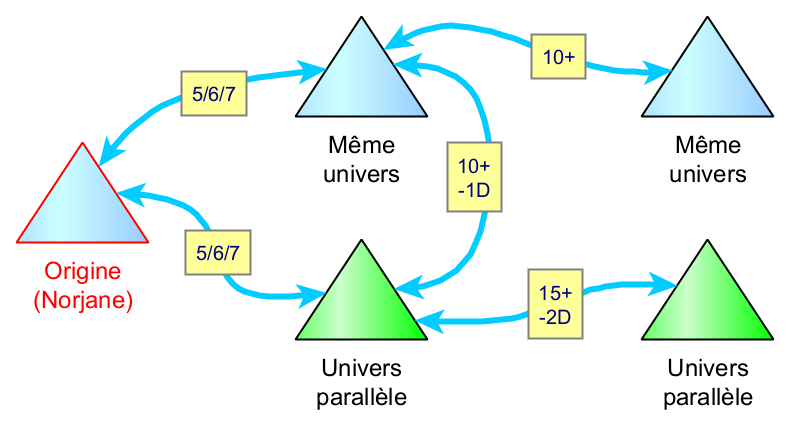
\includegraphics[scale=0.18]{mega-transit} & 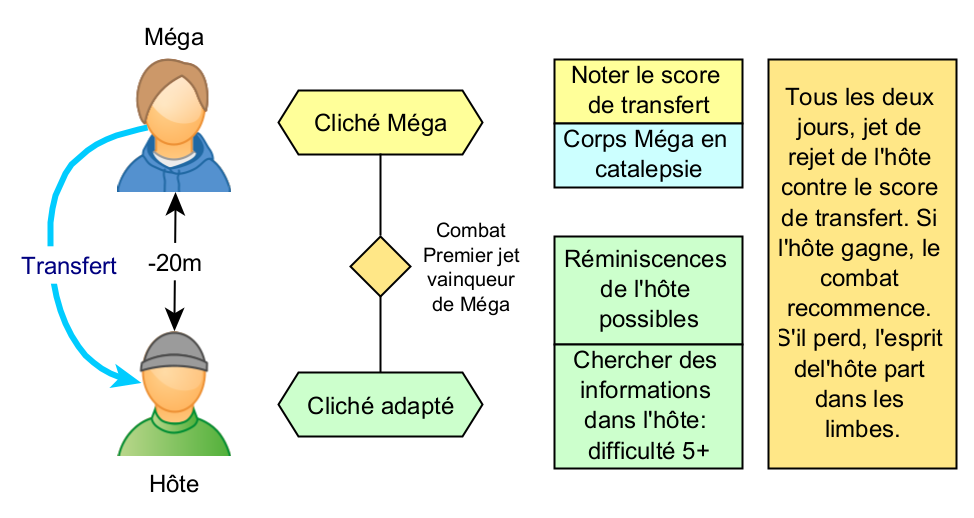
\includegraphics[scale=.16]{mega-transfert} \\
\end{tabular}}
\end{center}

%\mysubsection{Le Transit}

%\begin{wrapfigure}[lineheight]{position}{width}
%                   Nb de lignes / l c r / en fractions de linewidth
\begin{comment}
\begin{wrapfigure}[9]{l}{.5\linewidth}
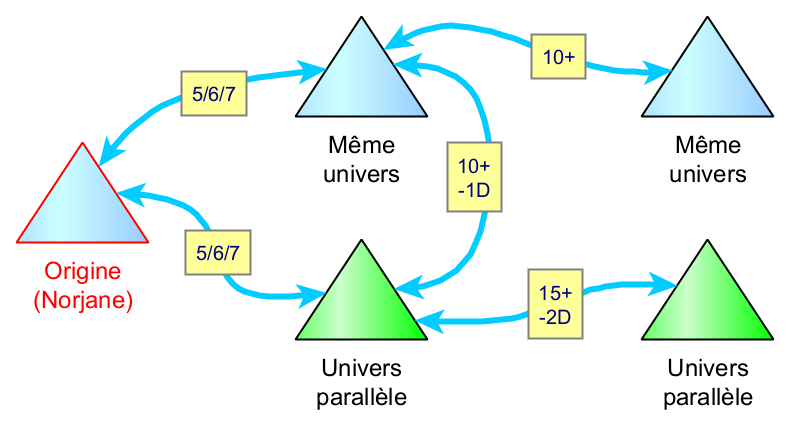
\includegraphics[scale=0.225]{mega-transit}
\end{wrapfigure}

\begin{wrapfigure}[8]{r}{.5\linewidth}
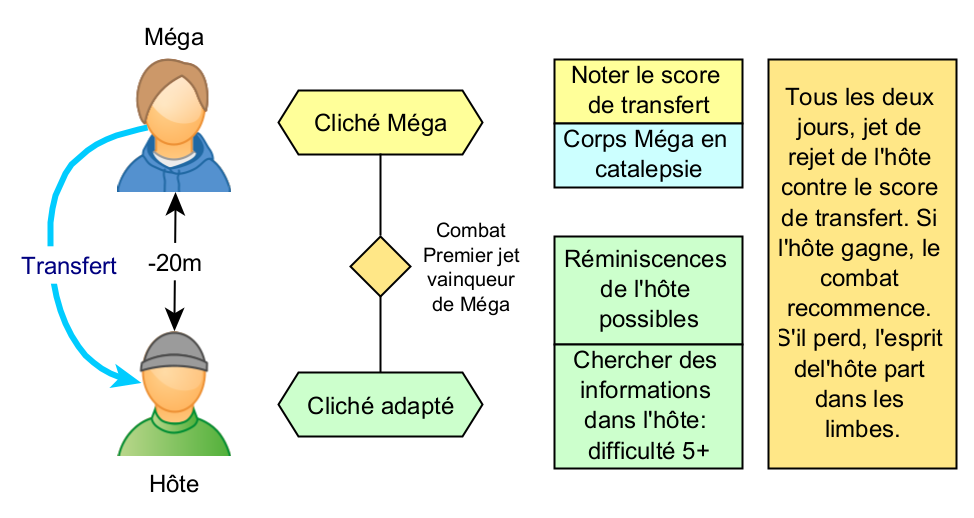
\includegraphics[scale=0.1]{mega-transfert}
\end{wrapfigure}
\end{comment}

%\begin{center}
%
\includegraphics[scale=0.5]{logo-orey}
%\end{center}

%======= mysection
% TODO licence
\vfill
\mysection{Licence}

\textit{Risus : The Anything RPG} est un jeu créé par S. John Ross. Les droits sont possédés par \href{https://risusrpg.com/}{Dave LeCompte} et \href{https://bigdicegames.com/}{Big Dice Games} Voir aussi la \href{https://drive.google.com/file/d/109_5S1oGDrGoXjVULVypIQQPnuxeTb5B/edit}{traduction française} de \href{https://www.legrog.org/biographies/tristan-lhomme}{Tristan Lhomme}.




\end{multicols*}



\end{document}
